% Options for packages loaded elsewhere
\PassOptionsToPackage{unicode}{hyperref}
\PassOptionsToPackage{hyphens}{url}
\PassOptionsToPackage{dvipsnames,svgnames*,x11names*}{xcolor}
%
\documentclass[
]{article}
\usepackage{amsmath,amssymb}
\usepackage{lmodern}
\usepackage{ifxetex,ifluatex}
\ifnum 0\ifxetex 1\fi\ifluatex 1\fi=0 % if pdftex
  \usepackage[T1]{fontenc}
  \usepackage[utf8]{inputenc}
  \usepackage{textcomp} % provide euro and other symbols
\else % if luatex or xetex
  \usepackage{unicode-math}
  \defaultfontfeatures{Scale=MatchLowercase}
  \defaultfontfeatures[\rmfamily]{Ligatures=TeX,Scale=1}
\fi
% Use upquote if available, for straight quotes in verbatim environments
\IfFileExists{upquote.sty}{\usepackage{upquote}}{}
\IfFileExists{microtype.sty}{% use microtype if available
  \usepackage[]{microtype}
  \UseMicrotypeSet[protrusion]{basicmath} % disable protrusion for tt fonts
}{}
\makeatletter
\@ifundefined{KOMAClassName}{% if non-KOMA class
  \IfFileExists{parskip.sty}{%
    \usepackage{parskip}
  }{% else
    \setlength{\parindent}{0pt}
    \setlength{\parskip}{6pt plus 2pt minus 1pt}}
}{% if KOMA class
  \KOMAoptions{parskip=half}}
\makeatother
\usepackage{xcolor}
\IfFileExists{xurl.sty}{\usepackage{xurl}}{} % add URL line breaks if available
\IfFileExists{bookmark.sty}{\usepackage{bookmark}}{\usepackage{hyperref}}
\hypersetup{
  pdftitle={Log of Crab body metrics - predicting the subspecies of crabs},
  pdfauthor={IJsbrand Pool, 403589},
  colorlinks=true,
  linkcolor=blue,
  filecolor=Maroon,
  citecolor=Blue,
  urlcolor=Blue,
  pdfcreator={LaTeX via pandoc}}
\urlstyle{same} % disable monospaced font for URLs
\usepackage[margin=1in]{geometry}
\usepackage{color}
\usepackage{fancyvrb}
\newcommand{\VerbBar}{|}
\newcommand{\VERB}{\Verb[commandchars=\\\{\}]}
\DefineVerbatimEnvironment{Highlighting}{Verbatim}{commandchars=\\\{\}}
% Add ',fontsize=\small' for more characters per line
\newenvironment{Shaded}{}{}
\newcommand{\AlertTok}[1]{\textcolor[rgb]{1.00,0.00,0.00}{#1}}
\newcommand{\AnnotationTok}[1]{\textcolor[rgb]{0.00,0.50,0.00}{#1}}
\newcommand{\AttributeTok}[1]{#1}
\newcommand{\BaseNTok}[1]{#1}
\newcommand{\BuiltInTok}[1]{#1}
\newcommand{\CharTok}[1]{\textcolor[rgb]{0.00,0.50,0.50}{#1}}
\newcommand{\CommentTok}[1]{\textcolor[rgb]{0.00,0.50,0.00}{#1}}
\newcommand{\CommentVarTok}[1]{\textcolor[rgb]{0.00,0.50,0.00}{#1}}
\newcommand{\ConstantTok}[1]{#1}
\newcommand{\ControlFlowTok}[1]{\textcolor[rgb]{0.00,0.00,1.00}{#1}}
\newcommand{\DataTypeTok}[1]{#1}
\newcommand{\DecValTok}[1]{#1}
\newcommand{\DocumentationTok}[1]{\textcolor[rgb]{0.00,0.50,0.00}{#1}}
\newcommand{\ErrorTok}[1]{\textcolor[rgb]{1.00,0.00,0.00}{\textbf{#1}}}
\newcommand{\ExtensionTok}[1]{#1}
\newcommand{\FloatTok}[1]{#1}
\newcommand{\FunctionTok}[1]{#1}
\newcommand{\ImportTok}[1]{#1}
\newcommand{\InformationTok}[1]{\textcolor[rgb]{0.00,0.50,0.00}{#1}}
\newcommand{\KeywordTok}[1]{\textcolor[rgb]{0.00,0.00,1.00}{#1}}
\newcommand{\NormalTok}[1]{#1}
\newcommand{\OperatorTok}[1]{#1}
\newcommand{\OtherTok}[1]{\textcolor[rgb]{1.00,0.25,0.00}{#1}}
\newcommand{\PreprocessorTok}[1]{\textcolor[rgb]{1.00,0.25,0.00}{#1}}
\newcommand{\RegionMarkerTok}[1]{#1}
\newcommand{\SpecialCharTok}[1]{\textcolor[rgb]{0.00,0.50,0.50}{#1}}
\newcommand{\SpecialStringTok}[1]{\textcolor[rgb]{0.00,0.50,0.50}{#1}}
\newcommand{\StringTok}[1]{\textcolor[rgb]{0.00,0.50,0.50}{#1}}
\newcommand{\VariableTok}[1]{#1}
\newcommand{\VerbatimStringTok}[1]{\textcolor[rgb]{0.00,0.50,0.50}{#1}}
\newcommand{\WarningTok}[1]{\textcolor[rgb]{0.00,0.50,0.00}{\textbf{#1}}}
\usepackage{graphicx}
\makeatletter
\def\maxwidth{\ifdim\Gin@nat@width>\linewidth\linewidth\else\Gin@nat@width\fi}
\def\maxheight{\ifdim\Gin@nat@height>\textheight\textheight\else\Gin@nat@height\fi}
\makeatother
% Scale images if necessary, so that they will not overflow the page
% margins by default, and it is still possible to overwrite the defaults
% using explicit options in \includegraphics[width, height, ...]{}
\setkeys{Gin}{width=\maxwidth,height=\maxheight,keepaspectratio}
% Set default figure placement to htbp
\makeatletter
\def\fps@figure{htbp}
\makeatother
\setlength{\emergencystretch}{3em} % prevent overfull lines
\providecommand{\tightlist}{%
  \setlength{\itemsep}{0pt}\setlength{\parskip}{0pt}}
\setcounter{secnumdepth}{5}
\usepackage{graphicx}
\usepackage{float}
\usepackage{booktabs}
\usepackage{longtable}
\usepackage{array}
\usepackage{multirow}
\usepackage{wrapfig}
\usepackage{float}
\usepackage{colortbl}
\usepackage{pdflscape}
\usepackage{tabu}
\usepackage{threeparttable}
\usepackage{threeparttablex}
\usepackage[normalem]{ulem}
\usepackage{makecell}
\usepackage{xcolor}
\ifluatex
  \usepackage{selnolig}  % disable illegal ligatures
\fi

\title{Log of Crab body metrics - predicting the subspecies of crabs}
\author{IJsbrand Pool, 403589}
\date{}

\begin{document}
\maketitle

{
\hypersetup{linkcolor=}
\setcounter{tocdepth}{2}
\tableofcontents
}
\newpage

\hypertarget{logbook-eda}{%
\section{Logbook EDA}\label{logbook-eda}}

\hypertarget{dataset-information}{%
\subsection{Dataset information}\label{dataset-information}}

The rock crab \emph{Leptograpsus variegatus}, is recorded as occurring
on a number of southern Pacific islands, the western coast of South
America, and the coasts of Australia south of the Tropic of Capricorn.
Mahon, using ecological studies which extended those of Shield, and a
genetical analysis based on an electrophoretic study, established the
specific distinctness of rock crabs of the blue and orange forms of the
genus \emph{Leptograpsus} which occur on the coasts of Australia. These
colour forms were previously regarded as morphs of \emph{L. variegatus.}

In an attempt to resolve this problem of identification, a morphological
study of the Western Australian species was undertaken. This paper
reports an exploratory data analysis of the data and a machine learning
algorithm to predict the species of the crab based on this data.

The dataset used is the crab body metrics dataset by Campbell, N.A. and
Mahon, R.J. (1974) A multivariate study of variation in two species of
rock crab of genus \emph{Leptograpsus}{[}1{]}. This data set contains
multiple morphological metrics of the bodies of \emph{L. variegatus.}
crabs, and the gender and color of the crab. The measured metrics are
the frontal lobe size, rear width, carapace length, carapace width and
body depth. All these values are in millimeters. There are 100 orange
and 100 blue crabs. 50 crabs of each gender per color of crab.

\hypertarget{research-question}{%
\subsubsection{Research question}\label{research-question}}

The goal of this project was to find out if the subspecies of a
\emph{Leptograpsus variegatus} was predictable.To find out if this is
possible, a research question had to be formulated. The research
question for this project is ``Can the species of a \emph{L.variegatus}
be determined based on some morphological measurements of its
carapace''. To answer this question, the data was first explored and
cleaned. Then, multiple machine learning algorithms were tested to find
what algorithm could be used best.

\newpage

\hypertarget{data-analysis}{%
\subsection{Data analysis}\label{data-analysis}}

\begin{Shaded}
\begin{Highlighting}[]
\CommentTok{\# Load in the data}
\NormalTok{myData }\OtherTok{\textless{}{-}} \FunctionTok{read.csv}\NormalTok{(}\StringTok{"datafiles/data.csv"}\NormalTok{)}

\CommentTok{\# Making the two separate subgroups}
\NormalTok{bluecrabs }\OtherTok{\textless{}{-}}\NormalTok{ myData[myData}\SpecialCharTok{$}\NormalTok{sp }\SpecialCharTok{==} \StringTok{"B"}\NormalTok{,]}
\NormalTok{orangecrabs }\OtherTok{\textless{}{-}}\NormalTok{ myData[myData}\SpecialCharTok{$}\NormalTok{sp }\SpecialCharTok{==} \StringTok{"O"}\NormalTok{,]}

\CommentTok{\# Creating the code book}
\NormalTok{column }\OtherTok{\textless{}{-}} \FunctionTok{colnames}\NormalTok{(myData)}
\NormalTok{description }\OtherTok{\textless{}{-}} \FunctionTok{c}\NormalTok{(}\StringTok{"Species"}\NormalTok{, }\StringTok{"Sex"}\NormalTok{, }\StringTok{"Index"}\NormalTok{, }\StringTok{"Frontal lobe size (mm)"}\NormalTok{, }\StringTok{"Rear width (mm)"}\NormalTok{,}
                 \StringTok{"Carapace length (mm)"}\NormalTok{, }\StringTok{"Carapace width (mm)"}\NormalTok{, }\StringTok{"Body depth (mm)"}\NormalTok{)}
\NormalTok{codebook }\OtherTok{\textless{}{-}} \FunctionTok{data.frame}\NormalTok{(column, description)}

\FunctionTok{kable}\NormalTok{(codebook, }\AttributeTok{caption =} \StringTok{"Codebook of the crab data set"}\NormalTok{) }\SpecialCharTok{\%\textgreater{}\%} 
\FunctionTok{kable\_styling}\NormalTok{(}\AttributeTok{font\_size =} \DecValTok{10}\NormalTok{, }\AttributeTok{latex\_options =} \StringTok{"hold\_position"}\NormalTok{)}
\end{Highlighting}
\end{Shaded}

\begin{table}[!h]

\caption{\label{tab:Reading data}Codebook of the crab data set}
\centering
\fontsize{10}{12}\selectfont
\begin{tabular}[t]{l|l}
\hline
column & description\\
\hline
sp & Species\\
\hline
sex & Sex\\
\hline
index & Index\\
\hline
FL & Frontal lobe size (mm)\\
\hline
RW & Rear width (mm)\\
\hline
CL & Carapace length (mm)\\
\hline
CW & Carapace width (mm)\\
\hline
BD & Body depth (mm)\\
\hline
\end{tabular}
\end{table}

After the data was loaded in, a code book with the attribute names and
their descriptions was generated, shown in table 1. To get a better view
of the measurements in the data set, a five number summary was created
for each attribute. These values are shown in table 2. The table shows
that the mean and the median are close in value for each column, meaning
that they all are normal distributions.

\begin{Shaded}
\begin{Highlighting}[]
\NormalTok{sumdat }\OtherTok{\textless{}{-}} \FunctionTok{summary}\NormalTok{(myData[}\DecValTok{4}\SpecialCharTok{:}\DecValTok{8}\NormalTok{])}
\NormalTok{sumdat }\OtherTok{\textless{}{-}} \FunctionTok{sub}\NormalTok{(}\StringTok{".*:"}\NormalTok{, }\StringTok{""}\NormalTok{, sumdat)}
\FunctionTok{rownames}\NormalTok{(sumdat) }\OtherTok{\textless{}{-}}  \FunctionTok{c}\NormalTok{(}\StringTok{"Minimum"}\NormalTok{, }\StringTok{"Q1"}\NormalTok{, }\StringTok{"Median"}\NormalTok{, }\StringTok{"Mean"}\NormalTok{, }\StringTok{"Q3"}\NormalTok{, }\StringTok{"Maximum"}\NormalTok{)}
\FunctionTok{colnames}\NormalTok{(sumdat) }\OtherTok{\textless{}{-}} \FunctionTok{c}\NormalTok{(}\StringTok{"Frontal Lobe"}\NormalTok{, }\StringTok{"Rear Width"}\NormalTok{, }\StringTok{"Carapace Length"}\NormalTok{, }\StringTok{"Carapace Width"}\NormalTok{, }\StringTok{"Body Depth"}\NormalTok{)}
\FunctionTok{kable}\NormalTok{(sumdat, }\AttributeTok{caption =} \StringTok{"Five number summaries of the morphological measurements."}\NormalTok{) }\SpecialCharTok{\%\textgreater{}\%} 
\FunctionTok{kable\_styling}\NormalTok{(}\AttributeTok{latex\_options =} \StringTok{"hold\_position"}\NormalTok{)}
\end{Highlighting}
\end{Shaded}

\begin{table}[!h]

\caption{\label{tab:summary}Five number summaries of the morphological measurements.}
\centering
\begin{tabular}[t]{l|l|l|l|l|l}
\hline
  & Frontal Lobe & Rear Width & Carapace Length & Carapace Width & Body Depth\\
\hline
Minimum & 7.20 & 6.50 & 14.70 & 17.10 & 6.10\\
\hline
Q1 & 12.90 & 11.00 & 27.27 & 31.50 & 11.40\\
\hline
Median & 15.55 & 12.80 & 32.10 & 36.80 & 13.90\\
\hline
Mean & 15.58 & 12.74 & 32.11 & 36.41 & 14.03\\
\hline
Q3 & 18.05 & 14.30 & 37.23 & 42.00 & 16.60\\
\hline
Maximum & 23.10 & 20.20 & 47.60 & 54.60 & 21.60\\
\hline
\end{tabular}
\end{table}

The data in its current form, is not ready for the use of a machine
learning algorithm, this is due to the Index column, some algorithms
will over fit their model by making use of this column, so this column
needs to be deleted to be able to verify the quality of the data
gathered. The species columns was also moved to the last column so it
would be used as the class attribute.

\begin{Shaded}
\begin{Highlighting}[]
\CommentTok{\# Cleaning the data by the removal of column Index.}
\NormalTok{clean\_data }\OtherTok{\textless{}{-}}\NormalTok{ myData[,}\FunctionTok{c}\NormalTok{(}\DecValTok{2}\NormalTok{,}\DecValTok{4}\SpecialCharTok{:}\FunctionTok{ncol}\NormalTok{(myData), }\DecValTok{1}\NormalTok{)]}
\CommentTok{\#write.csv(clean\_data, "datafiles/cleanedData.csv", row.names = F, col.names = F)}
\end{Highlighting}
\end{Shaded}

\newpage

\hypertarget{visualisation}{%
\subsection{Visualisation}\label{visualisation}}

\hypertarget{scatterplot-for-frontal-lobe-size-against-carapace-width}{%
\subsubsection{Scatterplot for frontal lobe size against carapace
width}\label{scatterplot-for-frontal-lobe-size-against-carapace-width}}

\begin{Shaded}
\begin{Highlighting}[]
\CommentTok{\#plot the Front lobe size against Carapace width}
\FunctionTok{ggplot}\NormalTok{(}\AttributeTok{data =}\NormalTok{ clean\_data,  }
\FunctionTok{aes}\NormalTok{(}\AttributeTok{x =}\NormalTok{ FL, }\AttributeTok{y =}\NormalTok{ CW)) }\SpecialCharTok{+} 
  \FunctionTok{geom\_jitter}\NormalTok{(}\AttributeTok{alpha =} \FloatTok{0.5}\NormalTok{, }\FunctionTok{aes}\NormalTok{(}\AttributeTok{colour =} \FunctionTok{factor}\NormalTok{(sp))) }\SpecialCharTok{+}  
  \FunctionTok{geom\_smooth}\NormalTok{(}\AttributeTok{method =} \StringTok{"lm"}\NormalTok{, }\AttributeTok{se =} \ConstantTok{FALSE}\NormalTok{, }\AttributeTok{formula=}\StringTok{"y\textasciitilde{}x"}\NormalTok{, }\FunctionTok{aes}\NormalTok{(}\AttributeTok{colour =}   \FunctionTok{factor}\NormalTok{(sp))) }\SpecialCharTok{+}
  \FunctionTok{scale\_color\_manual}\NormalTok{(}\AttributeTok{values=}\FunctionTok{c}\NormalTok{(}\StringTok{"Blue"}\NormalTok{,}\StringTok{"Orange"}\NormalTok{)) }\SpecialCharTok{+}
  \FunctionTok{ggtitle}\NormalTok{(}\StringTok{"Carapace width vs Frontal lobe size"}\NormalTok{) }\SpecialCharTok{+} 
  \FunctionTok{xlab}\NormalTok{(}\StringTok{"Frontal Lobe Size (mm)"}\NormalTok{) }\SpecialCharTok{+} \FunctionTok{ylab}\NormalTok{(}\StringTok{"Carapace Width (mm)"}\NormalTok{) }\SpecialCharTok{+}
  \FunctionTok{scale\_colour\_discrete}\NormalTok{(}\AttributeTok{name=}\StringTok{"Crab species"}\NormalTok{)}
\end{Highlighting}
\end{Shaded}

\begin{verbatim}
## Scale for 'colour' is already present. Adding another scale for 'colour',
## which will replace the existing scale.
\end{verbatim}

\begin{figure}[H]

{\centering 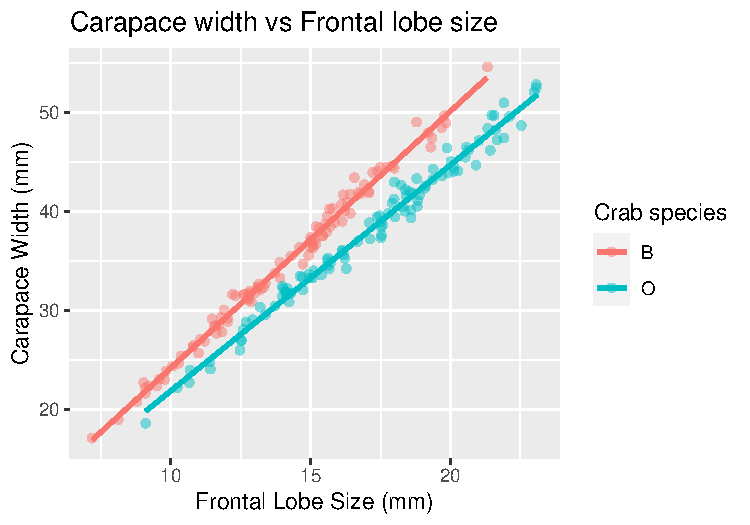
\includegraphics{Log_files/figure-latex/figure1-1} 

}

\caption{Spread of Front lobe size against Carapace width based on color}\label{fig:figure1}
\end{figure}

This plot plots the frontal lobe size against the carapace width of the
blue crabs as blue dots, and of the orange crabs as orange dots. It
shows that blue crabs on average have wider carapaces and shorter
frontal lobes, and that these attributes are somewhat correlated. This
could be a good indicator to determine the subspecies of the crab.
\newpage

\hypertarget{scatterplot-for-rear-width-against-carapace-length}{%
\subsubsection{Scatterplot for rear width against carapace
length}\label{scatterplot-for-rear-width-against-carapace-length}}

\begin{Shaded}
\begin{Highlighting}[]
\CommentTok{\#plot the Rear width against Carapace length}
\FunctionTok{ggplot}\NormalTok{() }\SpecialCharTok{+}
  \FunctionTok{geom\_point}\NormalTok{(}\AttributeTok{data =}\NormalTok{ myData[myData}\SpecialCharTok{$}\NormalTok{sp }\SpecialCharTok{==} \StringTok{"B"}\NormalTok{,], }\AttributeTok{mapping =} \FunctionTok{aes}\NormalTok{(}\AttributeTok{x =}\NormalTok{ RW, }\AttributeTok{y =}\NormalTok{ CL, }\AttributeTok{color =} \StringTok{\textquotesingle{}Blue\textquotesingle{}}\NormalTok{)) }\SpecialCharTok{+}
  \FunctionTok{geom\_point}\NormalTok{(}\AttributeTok{data =}\NormalTok{ myData[myData}\SpecialCharTok{$}\NormalTok{sp }\SpecialCharTok{==} \StringTok{"O"}\NormalTok{,], }\AttributeTok{mapping =} \FunctionTok{aes}\NormalTok{(}\AttributeTok{x =}\NormalTok{ RW, }\AttributeTok{y =}\NormalTok{ CL, }\AttributeTok{color =} \StringTok{\textquotesingle{}Orange\textquotesingle{}}\NormalTok{)) }\SpecialCharTok{+}
  \FunctionTok{scale\_color\_manual}\NormalTok{(}\AttributeTok{values=}\FunctionTok{c}\NormalTok{(}\StringTok{"\#4444EE"}\NormalTok{, }\StringTok{"\#E69F00"}\NormalTok{)) }\SpecialCharTok{+}
  \FunctionTok{labs}\NormalTok{(}\AttributeTok{x =} \StringTok{"Rear width (mm)"}\NormalTok{, }\AttributeTok{y =} \StringTok{"Carapace length (mm)"}\NormalTok{, }\AttributeTok{title=}\StringTok{\textquotesingle{}Rear width against Carapace length\textquotesingle{}}\NormalTok{)}
\end{Highlighting}
\end{Shaded}

\begin{figure}[H]

{\centering 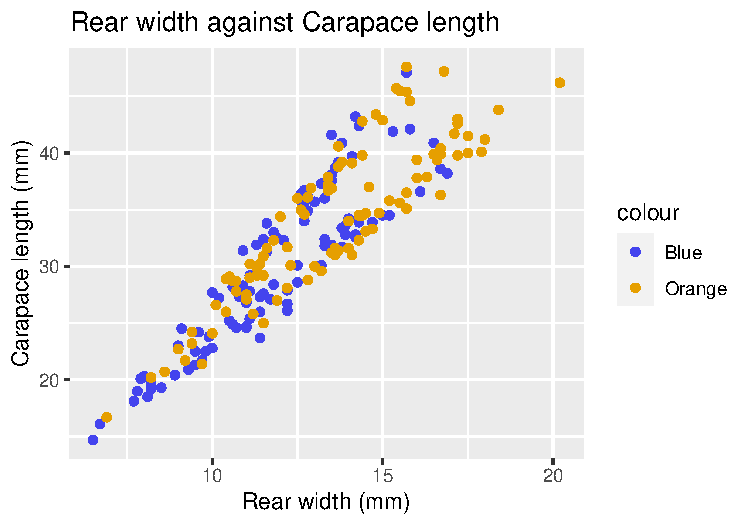
\includegraphics{Log_files/figure-latex/figure2-1} 

}

\caption{Spread of Rear width against Carapace length based on color}\label{fig:figure2}
\end{figure}

In this plot, the datapoints of the blue crabs are colored blue, and the
datapoints of the orange crabs colored orange again. This plot however,
does not show a clear difference between blue and orange crabs. Still
there are 2 separated groups, this means that these attributes are also
somewhat correlated and this could be investigated further. \newpage

\hypertarget{scatterplot-for-body-depth-against-carapace-width}{%
\subsubsection{Scatterplot for body depth against carapace
width}\label{scatterplot-for-body-depth-against-carapace-width}}

\begin{Shaded}
\begin{Highlighting}[]
\CommentTok{\#plot the Body depth against Carapace width}
\FunctionTok{ggplot}\NormalTok{() }\SpecialCharTok{+}
  \FunctionTok{geom\_point}\NormalTok{(}\AttributeTok{data =}\NormalTok{ myData[myData}\SpecialCharTok{$}\NormalTok{sp }\SpecialCharTok{==} \StringTok{"B"}\NormalTok{,], }\AttributeTok{mapping =} \FunctionTok{aes}\NormalTok{(}\AttributeTok{x =}\NormalTok{ BD, }\AttributeTok{y =}\NormalTok{ CW, }\AttributeTok{color =} \StringTok{\textquotesingle{}Blue\textquotesingle{}}\NormalTok{)) }\SpecialCharTok{+}
  \FunctionTok{geom\_point}\NormalTok{(}\AttributeTok{data =}\NormalTok{ myData[myData}\SpecialCharTok{$}\NormalTok{sp }\SpecialCharTok{==} \StringTok{"O"}\NormalTok{,], }\AttributeTok{mapping =} \FunctionTok{aes}\NormalTok{(}\AttributeTok{x =}\NormalTok{ BD, }\AttributeTok{y =}\NormalTok{ CW, }\AttributeTok{color =} \StringTok{\textquotesingle{}Orange\textquotesingle{}}\NormalTok{)) }\SpecialCharTok{+}
  \FunctionTok{scale\_color\_manual}\NormalTok{(}\AttributeTok{values=}\FunctionTok{c}\NormalTok{(}\StringTok{"\#4444EE"}\NormalTok{, }\StringTok{"\#E69F00"}\NormalTok{)) }\SpecialCharTok{+}
  \FunctionTok{labs}\NormalTok{(}\AttributeTok{x =} \StringTok{"Body depth (mm)"}\NormalTok{, }\AttributeTok{y =} \StringTok{"Carapace width (mm)"}\NormalTok{, }\AttributeTok{title=}\StringTok{\textquotesingle{}Body depth against Carapace width\textquotesingle{}}\NormalTok{)}
\end{Highlighting}
\end{Shaded}

\begin{figure}[H]

{\centering 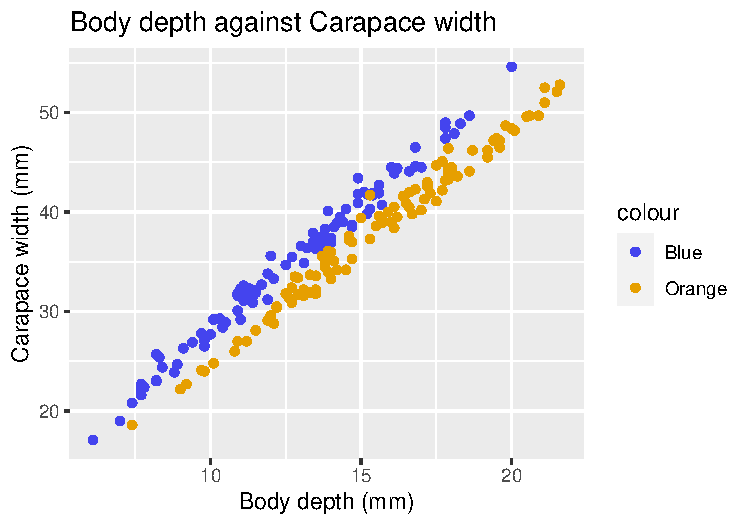
\includegraphics{Log_files/figure-latex/figure3-1} 

}

\caption{Spread of Body depth against Carapace width based on color}\label{fig:figure3}
\end{figure}

In this plot, again the data points were colored to represent the color
of the crab. This plot also shows that blue crabs on average have wider
carapaces, but that orange crabs tend to have deeper bodies, and that
these attributes are somewhat correlated. This could also be a good
indicator to determine the subspecies of the crab, though its less clear
than figure 1. \newpage

\begin{Shaded}
\begin{Highlighting}[]
\NormalTok{densityplot1 }\OtherTok{\textless{}{-}} \FunctionTok{ggplot}\NormalTok{(clean\_data, }\FunctionTok{aes}\NormalTok{(FL), }\AttributeTok{alpha =} \FloatTok{0.5}\NormalTok{) }\SpecialCharTok{+} \FunctionTok{geom\_density}\NormalTok{(}\FunctionTok{aes}\NormalTok{(}\AttributeTok{col =}\NormalTok{ sex, }\AttributeTok{fill=}\NormalTok{sex), }
                                                                        \AttributeTok{alpha =} \FloatTok{0.5}\NormalTok{) }\SpecialCharTok{+}
\FunctionTok{ggtitle}\NormalTok{(}\StringTok{"FL"}\NormalTok{) }\SpecialCharTok{+} \FunctionTok{ylab}\NormalTok{(}\StringTok{"Density"}\NormalTok{)}


\NormalTok{densityplot2 }\OtherTok{\textless{}{-}} \FunctionTok{ggplot}\NormalTok{(clean\_data, }\FunctionTok{aes}\NormalTok{(RW), }\AttributeTok{alpha =} \FloatTok{0.5}\NormalTok{) }\SpecialCharTok{+} \FunctionTok{geom\_density}\NormalTok{(}\FunctionTok{aes}\NormalTok{(}\AttributeTok{col =}\NormalTok{ sex, }\AttributeTok{fill=}\NormalTok{sex), }
                                                                        \AttributeTok{alpha =} \FloatTok{0.5}\NormalTok{) }\SpecialCharTok{+}
\FunctionTok{ggtitle}\NormalTok{(}\StringTok{"RW"}\NormalTok{) }\SpecialCharTok{+} \FunctionTok{ylab}\NormalTok{(}\StringTok{"Density"}\NormalTok{)}

\NormalTok{densityplot3 }\OtherTok{\textless{}{-}} \FunctionTok{ggplot}\NormalTok{(clean\_data, }\FunctionTok{aes}\NormalTok{(CL), }\AttributeTok{alpha =} \FloatTok{0.5}\NormalTok{) }\SpecialCharTok{+} \FunctionTok{geom\_density}\NormalTok{(}\FunctionTok{aes}\NormalTok{(}\AttributeTok{col =}\NormalTok{ sex, }\AttributeTok{fill=}\NormalTok{ sex), }
                                                                        \AttributeTok{alpha =} \FloatTok{0.5}\NormalTok{) }\SpecialCharTok{+}
\FunctionTok{ggtitle}\NormalTok{(}\StringTok{"CL"}\NormalTok{) }\SpecialCharTok{+} \FunctionTok{ylab}\NormalTok{(}\StringTok{"Density"}\NormalTok{)}

\NormalTok{densityplot4 }\OtherTok{\textless{}{-}} \FunctionTok{ggplot}\NormalTok{(clean\_data, }\FunctionTok{aes}\NormalTok{(CW), }\AttributeTok{alpha =} \FloatTok{0.5}\NormalTok{) }\SpecialCharTok{+} \FunctionTok{geom\_density}\NormalTok{(}\FunctionTok{aes}\NormalTok{(}\AttributeTok{col =}\NormalTok{ sex, }\AttributeTok{fill=}\NormalTok{sex), }
                                                                        \AttributeTok{alpha =} \FloatTok{0.5}\NormalTok{) }\SpecialCharTok{+}
\FunctionTok{ggtitle}\NormalTok{(}\StringTok{"CW"}\NormalTok{) }\SpecialCharTok{+} \FunctionTok{ylab}\NormalTok{(}\StringTok{"Density"}\NormalTok{)}

\NormalTok{densityplot5 }\OtherTok{\textless{}{-}} \FunctionTok{ggplot}\NormalTok{(clean\_data, }\FunctionTok{aes}\NormalTok{(BD), }\AttributeTok{alpha =} \FloatTok{0.5}\NormalTok{) }\SpecialCharTok{+} \FunctionTok{geom\_density}\NormalTok{(}\FunctionTok{aes}\NormalTok{(}\AttributeTok{col =}\NormalTok{ sex,}\AttributeTok{fill=}\NormalTok{ sex), }
                                                                        \AttributeTok{alpha =} \FloatTok{0.5}\NormalTok{) }\SpecialCharTok{+}
\FunctionTok{ggtitle}\NormalTok{(}\StringTok{"BD"}\NormalTok{) }\SpecialCharTok{+} \FunctionTok{ylab}\NormalTok{(}\StringTok{"Density"}\NormalTok{)}

\NormalTok{densityplots }\OtherTok{\textless{}{-}} \FunctionTok{ggarrange}\NormalTok{(densityplot1, densityplot2, densityplot3, densityplot4, densityplot5,}
                   \AttributeTok{ncol =} \DecValTok{2}\NormalTok{, }\AttributeTok{nrow =} \DecValTok{3}\NormalTok{)}

\NormalTok{title }\OtherTok{\textless{}{-}} \FunctionTok{expression}\NormalTok{(}\FunctionTok{atop}\NormalTok{(}\FunctionTok{bold}\NormalTok{(}\StringTok{"Expression data"}\NormalTok{), }
         \FunctionTok{scriptstyle}\NormalTok{(}\FunctionTok{paste}\NormalTok{(}\StringTok{"Density plots of all the morhpological measurements compared to sex"}\NormalTok{))))}
\FunctionTok{annotate\_figure}\NormalTok{(densityplots,}
                \AttributeTok{top=}\FunctionTok{text\_grob}\NormalTok{(title))}
\end{Highlighting}
\end{Shaded}

\begin{figure}[H]

{\centering 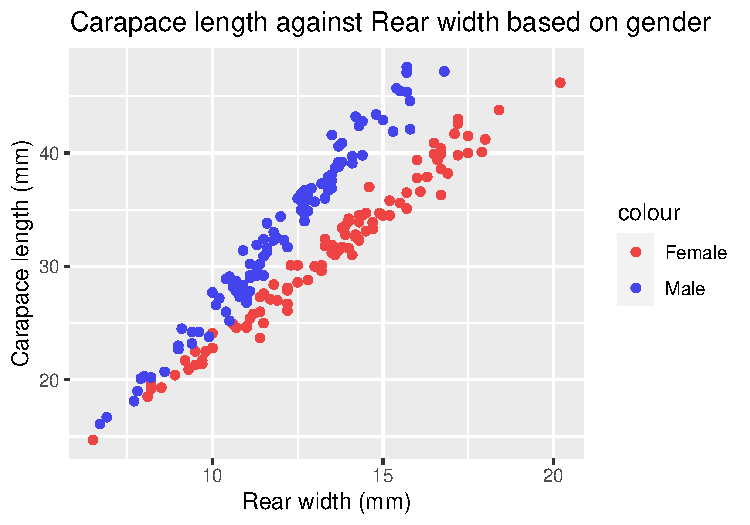
\includegraphics{Log_files/figure-latex/figure4-1} 

}

\caption{Checking if the gender makes a difference}\label{fig:figure4}
\end{figure}

As seen in the density distribution of figure four, there indeed seems
to be a difference within the groups if they are divided by the male and
females of the group.

In figure 4.1 the frontal lobe size in millimeters is plotted against
the gender of the crabs, here it is clearly visible that there doesn't
seem to be much difference in the frontal lobe size between the genders,
the only difference that can be seen here appears to be in the the
smaller measurements of the frontal lobe size, slightly indicating that
the females might have a smaller frontal lobe size in general then
males, this however cannot be confirmed from this density plot.

In figure 4.2 the Rear width in millimeters is plotted against the
gender of the crabs, here it can be seen that the female crabs appear to
have a bigger rear width then the male crabs, it could be that one
colour species has a larger rear width, but the most plausible reason
for this is that genetically speaking the female crab has a larger rear
width.

In figure 4.3 the Carapace length in millimeters is shown here against
the gender of the crabs, here similar to figure 4.1 there do not seem to
be many differences apart from the fact that more females appear to have
a carapace length of around 30 á 35 millimeters in length, this however
does not seem significant, and that a small portion of the male crabs
seem to have a larger carapace length then the females, but since this
doesn't seem like a mayority this could just be an anomaly.

In figure 4.4 the Carapace width is shown, measured in millimeters,
plotted against the gender of the crabs similar to the figure 4.3 there
do not seem to be a lot of differences, apart from the males where a
small portion seem to have a larger carapace width then the females,
this is however again a small portion so it may be insignificant.

In figure 4.5 the Body depth in millimeters is shown, this is plotted
against the gender of the crabs, here the distributions appear similar,
making is seem like gender does not affect body depth what so ever.

One thing that is noticeable here is the distributions of the female
crabs, these appear to be more of a normal distribution then the male
crabs, which can be due to coincidence since it is a small data set, but
it can also be that the body of a female crab is more normally
distributed then the body of its male counterpart.

\begin{Shaded}
\begin{Highlighting}[]
\NormalTok{corr }\OtherTok{\textless{}{-}} \FunctionTok{round}\NormalTok{(}\FunctionTok{cor}\NormalTok{(clean\_data[}\DecValTok{2}\SpecialCharTok{:}\DecValTok{6}\NormalTok{]), }\DecValTok{2}\NormalTok{)}

\CommentTok{\# Plot}
\FunctionTok{ggcorrplot}\NormalTok{(corr, }\AttributeTok{hc.order =} \ConstantTok{TRUE}\NormalTok{, }
           \AttributeTok{type =} \StringTok{"lower"}\NormalTok{, }
           \AttributeTok{lab =} \ConstantTok{TRUE}\NormalTok{, }
           \AttributeTok{lab\_size =} \DecValTok{3}\NormalTok{, }
           \AttributeTok{method=}\StringTok{"circle"}\NormalTok{, }
           \AttributeTok{colors =} \FunctionTok{c}\NormalTok{(}\StringTok{"tomato2"}\NormalTok{, }\StringTok{"white"}\NormalTok{, }\StringTok{"springgreen3"}\NormalTok{), }
           \AttributeTok{title=}\StringTok{"Correlogram of the crabs"}\NormalTok{, }
           \AttributeTok{ggtheme=}\NormalTok{theme\_bw)}
\end{Highlighting}
\end{Shaded}

\begin{center}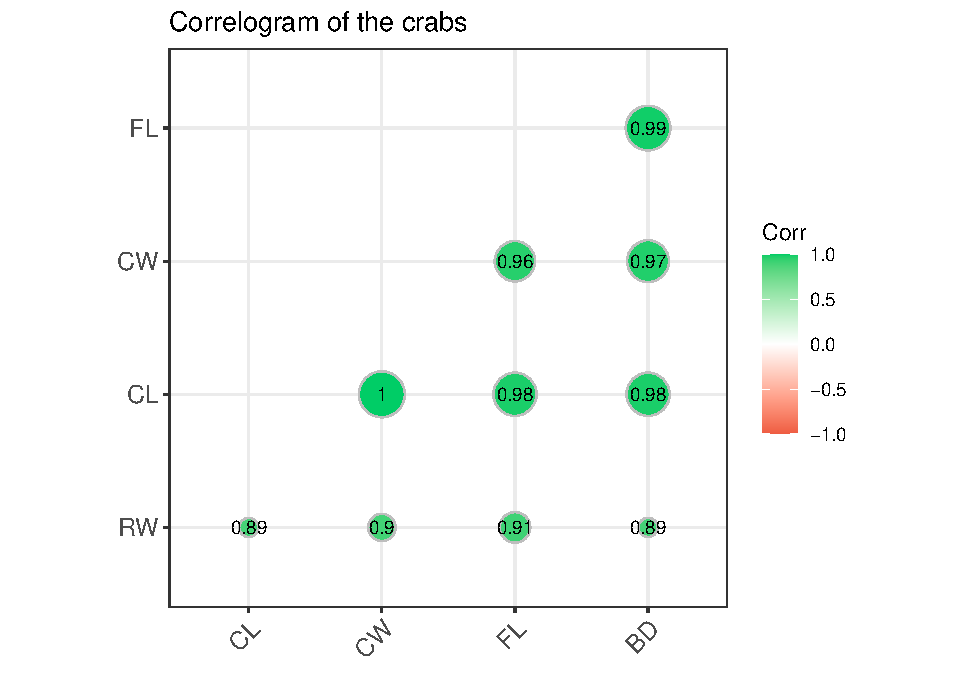
\includegraphics{Log_files/figure-latex/correlogram-1} \end{center}

In the plot above the correlation between all the numerical elements of
the data set are shown, this has been done to be able to answer the
previously arisen question whether or not the data is correlated.

As seen in the plot above, the data inside the data set does indeed seem
to correlate which supports the earlier findings, this could mean that
there is more then one good attribute to be able to confidently support
the investigation of the research question

\begin{Shaded}
\begin{Highlighting}[]
\NormalTok{orangedensityplot1 }\OtherTok{\textless{}{-}} \FunctionTok{ggplot}\NormalTok{(orangecrabs, }\FunctionTok{aes}\NormalTok{(FL), }\AttributeTok{alpha =} \FloatTok{0.5}\NormalTok{) }\SpecialCharTok{+}
  \FunctionTok{geom\_density}\NormalTok{(}\FunctionTok{aes}\NormalTok{(}\AttributeTok{col =}\NormalTok{ sex, }\AttributeTok{fill=}\NormalTok{sex), }\AttributeTok{alpha =} \FloatTok{0.5}\NormalTok{) }\SpecialCharTok{+}
\FunctionTok{ggtitle}\NormalTok{(}\StringTok{"FL"}\NormalTok{) }\SpecialCharTok{+} \FunctionTok{ylab}\NormalTok{(}\StringTok{"Density"}\NormalTok{)}

\NormalTok{orangedensityplot2 }\OtherTok{\textless{}{-}} \FunctionTok{ggplot}\NormalTok{(orangecrabs, }\FunctionTok{aes}\NormalTok{(RW), }\AttributeTok{alpha =} \FloatTok{0.5}\NormalTok{) }\SpecialCharTok{+}
  \FunctionTok{geom\_density}\NormalTok{(}\FunctionTok{aes}\NormalTok{(}\AttributeTok{col =}\NormalTok{ sex, }\AttributeTok{fill=}\NormalTok{sex), }\AttributeTok{alpha =} \FloatTok{0.5}\NormalTok{) }\SpecialCharTok{+}
\FunctionTok{ggtitle}\NormalTok{(}\StringTok{"RW"}\NormalTok{) }\SpecialCharTok{+} \FunctionTok{ylab}\NormalTok{(}\StringTok{"Density"}\NormalTok{)}

\NormalTok{orangedensityplot3 }\OtherTok{\textless{}{-}} \FunctionTok{ggplot}\NormalTok{(orangecrabs, }\FunctionTok{aes}\NormalTok{(CL), }\AttributeTok{alpha =} \FloatTok{0.5}\NormalTok{) }\SpecialCharTok{+}
  \FunctionTok{geom\_density}\NormalTok{(}\FunctionTok{aes}\NormalTok{(}\AttributeTok{col =}\NormalTok{ sex, }\AttributeTok{fill=}\NormalTok{ sex), }\AttributeTok{alpha =} \FloatTok{0.5}\NormalTok{) }\SpecialCharTok{+}
\FunctionTok{ggtitle}\NormalTok{(}\StringTok{"CL"}\NormalTok{) }\SpecialCharTok{+} \FunctionTok{ylab}\NormalTok{(}\StringTok{"Density"}\NormalTok{)}

\NormalTok{orangedensityplot4 }\OtherTok{\textless{}{-}} \FunctionTok{ggplot}\NormalTok{(orangecrabs, }\FunctionTok{aes}\NormalTok{(CW), }\AttributeTok{alpha =} \FloatTok{0.5}\NormalTok{) }\SpecialCharTok{+}
  \FunctionTok{geom\_density}\NormalTok{(}\FunctionTok{aes}\NormalTok{(}\AttributeTok{col =}\NormalTok{ sex, }\AttributeTok{fill=}\NormalTok{sex), }\AttributeTok{alpha =} \FloatTok{0.5}\NormalTok{) }\SpecialCharTok{+}
\FunctionTok{ggtitle}\NormalTok{(}\StringTok{"CW"}\NormalTok{) }\SpecialCharTok{+} \FunctionTok{ylab}\NormalTok{(}\StringTok{"Density"}\NormalTok{)}

\NormalTok{orangedensityplot5 }\OtherTok{\textless{}{-}} \FunctionTok{ggplot}\NormalTok{(orangecrabs, }\FunctionTok{aes}\NormalTok{(BD), }\AttributeTok{alpha =} \FloatTok{0.5}\NormalTok{) }\SpecialCharTok{+}
  \FunctionTok{geom\_density}\NormalTok{(}\FunctionTok{aes}\NormalTok{(}\AttributeTok{col =}\NormalTok{ sex,}\AttributeTok{fill=}\NormalTok{ sex), }\AttributeTok{alpha =} \FloatTok{0.5}\NormalTok{) }\SpecialCharTok{+}
\FunctionTok{ggtitle}\NormalTok{(}\StringTok{"BD"}\NormalTok{) }\SpecialCharTok{+} \FunctionTok{ylab}\NormalTok{(}\StringTok{"Density"}\NormalTok{)}

\NormalTok{orangedensityplots }\OtherTok{\textless{}{-}} \FunctionTok{ggarrange}\NormalTok{(orangedensityplot1, orangedensityplot2, orangedensityplot3,}
\NormalTok{                                orangedensityplot4, orangedensityplot5, }\AttributeTok{ncol =} \DecValTok{2}\NormalTok{, }\AttributeTok{nrow =} \DecValTok{3}\NormalTok{)}

\NormalTok{title }\OtherTok{\textless{}{-}} \FunctionTok{expression}\NormalTok{(}\FunctionTok{atop}\NormalTok{(}\FunctionTok{bold}\NormalTok{(}\StringTok{"Expression data"}\NormalTok{), }
        \FunctionTok{scriptstyle}\NormalTok{(}\FunctionTok{paste}\NormalTok{(}\StringTok{"Density plots of all the morhpological measurements compared to sex"}\NormalTok{))))}
\FunctionTok{annotate\_figure}\NormalTok{(orangedensityplots,}
                \AttributeTok{top=}\FunctionTok{text\_grob}\NormalTok{(title))}
\end{Highlighting}
\end{Shaded}

\begin{figure}[H]

{\centering 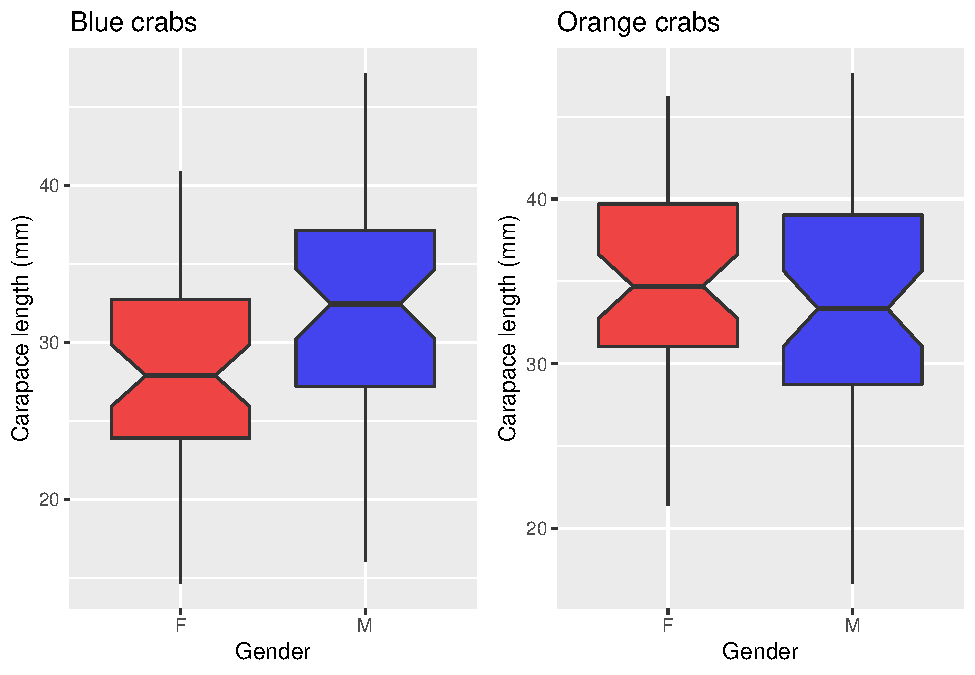
\includegraphics{Log_files/figure-latex/figure6-1} 

}

\caption{Checking if the gender makes a difference}\label{fig:figure6}
\end{figure}

As seen in figure six, the orange crabs their morphological measurements
have been taken to be able to see if the sex matters when it comes to
the colours of the crabs,

\begin{Shaded}
\begin{Highlighting}[]
\NormalTok{bluedensityplot1 }\OtherTok{\textless{}{-}} \FunctionTok{ggplot}\NormalTok{(bluecrabs, }\FunctionTok{aes}\NormalTok{(FL), }\AttributeTok{alpha =} \FloatTok{0.5}\NormalTok{) }\SpecialCharTok{+} 
  \FunctionTok{geom\_density}\NormalTok{(}\FunctionTok{aes}\NormalTok{(}\AttributeTok{col =}\NormalTok{ sex, }\AttributeTok{fill=}\NormalTok{sex), }\AttributeTok{alpha =} \FloatTok{0.5}\NormalTok{) }\SpecialCharTok{+}
\FunctionTok{ggtitle}\NormalTok{(}\StringTok{"FL"}\NormalTok{) }\SpecialCharTok{+} \FunctionTok{ylab}\NormalTok{(}\StringTok{"Density"}\NormalTok{)}

\NormalTok{bluedensityplot2 }\OtherTok{\textless{}{-}} \FunctionTok{ggplot}\NormalTok{(bluecrabs, }\FunctionTok{aes}\NormalTok{(RW), }\AttributeTok{alpha =} \FloatTok{0.5}\NormalTok{) }\SpecialCharTok{+} 
  \FunctionTok{geom\_density}\NormalTok{(}\FunctionTok{aes}\NormalTok{(}\AttributeTok{col =}\NormalTok{ sex, }\AttributeTok{fill=}\NormalTok{sex), }\AttributeTok{alpha =} \FloatTok{0.5}\NormalTok{) }\SpecialCharTok{+}
\FunctionTok{ggtitle}\NormalTok{(}\StringTok{"RW"}\NormalTok{) }\SpecialCharTok{+} \FunctionTok{ylab}\NormalTok{(}\StringTok{"Density"}\NormalTok{)}

\NormalTok{bluedensityplot3 }\OtherTok{\textless{}{-}} \FunctionTok{ggplot}\NormalTok{(bluecrabs, }\FunctionTok{aes}\NormalTok{(CL), }\AttributeTok{alpha =} \FloatTok{0.5}\NormalTok{) }\SpecialCharTok{+} 
  \FunctionTok{geom\_density}\NormalTok{(}\FunctionTok{aes}\NormalTok{(}\AttributeTok{col =}\NormalTok{ sex, }\AttributeTok{fill=}\NormalTok{ sex), }\AttributeTok{alpha =} \FloatTok{0.5}\NormalTok{) }\SpecialCharTok{+}
\FunctionTok{ggtitle}\NormalTok{(}\StringTok{"CL"}\NormalTok{) }\SpecialCharTok{+} \FunctionTok{ylab}\NormalTok{(}\StringTok{"Density"}\NormalTok{)}

\NormalTok{bluedensityplot4 }\OtherTok{\textless{}{-}} \FunctionTok{ggplot}\NormalTok{(bluecrabs, }\FunctionTok{aes}\NormalTok{(CW), }\AttributeTok{alpha =} \FloatTok{0.5}\NormalTok{) }\SpecialCharTok{+}
  \FunctionTok{geom\_density}\NormalTok{(}\FunctionTok{aes}\NormalTok{(}\AttributeTok{col =}\NormalTok{ sex, }\AttributeTok{fill=}\NormalTok{sex), }\AttributeTok{alpha =} \FloatTok{0.5}\NormalTok{) }\SpecialCharTok{+}
\FunctionTok{ggtitle}\NormalTok{(}\StringTok{"CW"}\NormalTok{) }\SpecialCharTok{+} \FunctionTok{ylab}\NormalTok{(}\StringTok{"Density"}\NormalTok{)}

\NormalTok{bluedensityplot5 }\OtherTok{\textless{}{-}} \FunctionTok{ggplot}\NormalTok{(bluecrabs, }\FunctionTok{aes}\NormalTok{(BD), }\AttributeTok{alpha =} \FloatTok{0.5}\NormalTok{) }\SpecialCharTok{+} 
  \FunctionTok{geom\_density}\NormalTok{(}\FunctionTok{aes}\NormalTok{(}\AttributeTok{col =}\NormalTok{ sex,}\AttributeTok{fill=}\NormalTok{ sex), }\AttributeTok{alpha =} \FloatTok{0.5}\NormalTok{) }\SpecialCharTok{+}
\FunctionTok{ggtitle}\NormalTok{(}\StringTok{"BD"}\NormalTok{) }\SpecialCharTok{+} \FunctionTok{ylab}\NormalTok{(}\StringTok{"Density"}\NormalTok{)}

\NormalTok{bluedensityplots }\OtherTok{\textless{}{-}} \FunctionTok{ggarrange}\NormalTok{(bluedensityplot1, bluedensityplot2, bluedensityplot3,}
\NormalTok{                              bluedensityplot4, bluedensityplot5,}\AttributeTok{ncol =} \DecValTok{2}\NormalTok{, }\AttributeTok{nrow =} \DecValTok{3}\NormalTok{)}

\NormalTok{title }\OtherTok{\textless{}{-}} \FunctionTok{expression}\NormalTok{(}\FunctionTok{atop}\NormalTok{(}\FunctionTok{bold}\NormalTok{(}\StringTok{"Expression data"}\NormalTok{), }
        \FunctionTok{scriptstyle}\NormalTok{(}\FunctionTok{paste}\NormalTok{(}\StringTok{"Density plots of all the morhpological measurements compared to sex"}\NormalTok{))))}
\FunctionTok{annotate\_figure}\NormalTok{(bluedensityplots,}
                \AttributeTok{top=}\FunctionTok{text\_grob}\NormalTok{(title))}
\end{Highlighting}
\end{Shaded}

\begin{center}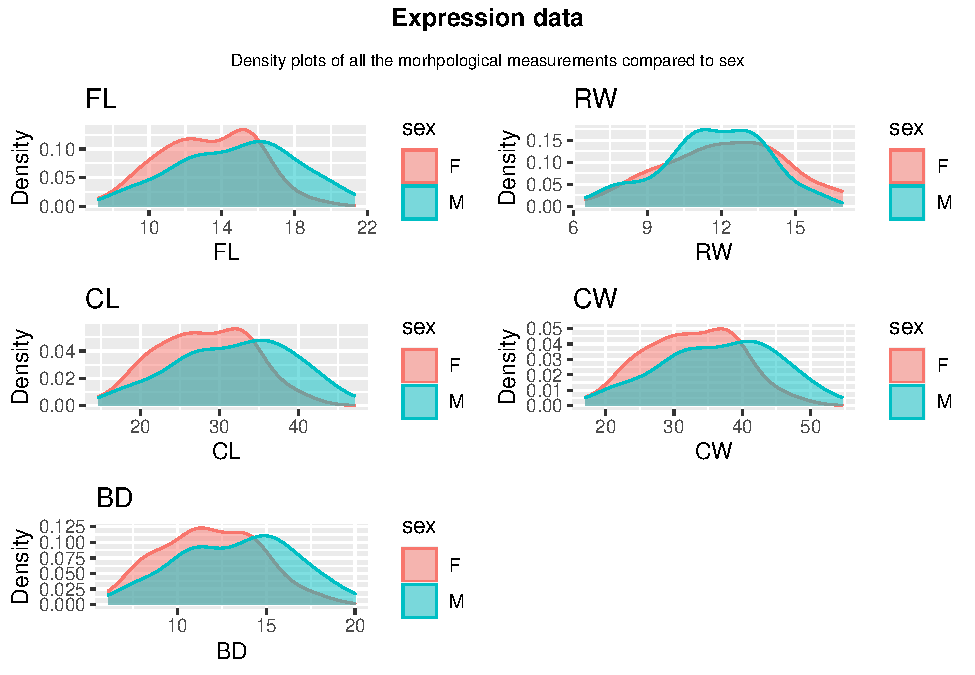
\includegraphics{Log_files/figure-latex/figure 7-1} \end{center}

In figure six and seven the morphological variables of both color crabs
have been put into a density plot to see if there is any correlation
there, here it is however clearly visible these two separate colors
differ in their measurements. As can be seen in figure six: There are no
real differences with the morphological measurements for the orange
crabs, apart from the rear width, and here the females are noted to have
a larger rear width, apart from that some males appear to be on the
lager side of the spectrum in the density plot, but this does not seem
significant enough that it is to be mentioned. The orange crabs also
seem to have somewhat of a normal distribution or bell curve when it
comes to their measurements, this could indicate that they are either
smaller or their morphological components are more formed to each other.

In figure seven the blue crabs are depicted, here differing from figure
six, the male crabs of the blue species seem to be bigger in almost all
aspects of the morphological components apart from rear width, this
would indicate that for this species the male variant is bigger then the
female variant, how ever, this is a data set with only 100 crabs per
species and for a correct distribution a much larger sample size should
be taken. For the carapace length, it seems that for this species alone
it would be very good to be determined if the crab was of significant
size, which species it would belong to. To see if this would work with a
machine learning algorithm, further testing will need to be done.

\hypertarget{pca-plot}{%
\subsubsection{PCA plot}\label{pca-plot}}

\begin{Shaded}
\begin{Highlighting}[]
\NormalTok{res.pca }\OtherTok{\textless{}{-}} \FunctionTok{PCA}\NormalTok{(myData[}\DecValTok{4}\SpecialCharTok{:}\FunctionTok{ncol}\NormalTok{(myData)], }\AttributeTok{ncp =} \DecValTok{5}\NormalTok{, }\AttributeTok{graph =} \ConstantTok{FALSE}\NormalTok{)}

\FunctionTok{fviz\_pca\_var}\NormalTok{(res.pca, }\AttributeTok{col.var =} \StringTok{"cos2"}\NormalTok{,}
             \AttributeTok{gradient.cols =} \FunctionTok{c}\NormalTok{(}\StringTok{"\#00AFBB"}\NormalTok{, }\StringTok{"\#E7B800"}\NormalTok{, }\StringTok{"\#FC4E07"}\NormalTok{), }
             \AttributeTok{repel =} \ConstantTok{TRUE}\NormalTok{)}
\end{Highlighting}
\end{Shaded}

\begin{center}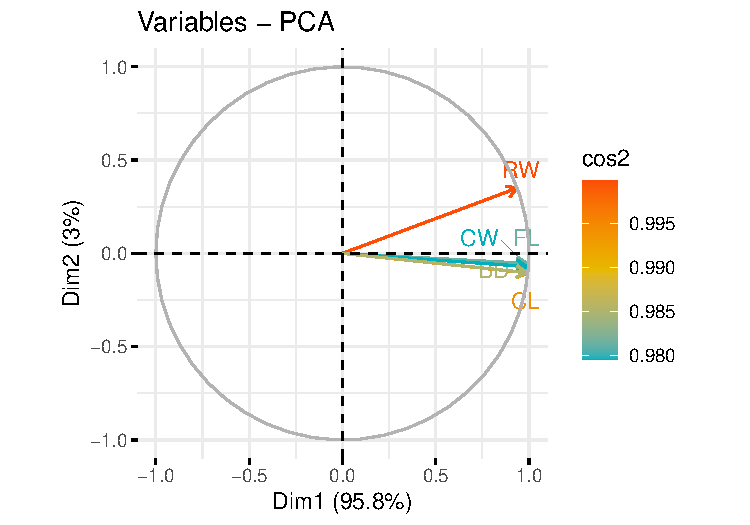
\includegraphics{Log_files/figure-latex/pca-1} \end{center}

This PCA plot was created to show the correlation between all variables.
This PCA plot shows that the variables are highly correlated. The least
correlated variable is the Rear width. This vector has the largest angle
with the Carapace length, the same two variables that were used to
discover the difference in carapace length distribution between the
genders.

\newpage

\hypertarget{machine-learning}{%
\subsection{Machine learning}\label{machine-learning}}

\hypertarget{cleaning}{%
\subsubsection{cleaning}\label{cleaning}}

Before machine learning can be used, the data must first be cleaned. In
its current form, the data is not ready for machine learning. Because of
the id column, some of the machine learning algorithms overfit their
model by using this column. So this column should be removed first. The
species columns was also moved to the last column so it would be used as
the class attribute.

\begin{Shaded}
\begin{Highlighting}[]
\NormalTok{clean\_data }\OtherTok{\textless{}{-}}\NormalTok{ myData[,}\FunctionTok{c}\NormalTok{(}\DecValTok{2}\NormalTok{,}\DecValTok{4}\SpecialCharTok{:}\FunctionTok{ncol}\NormalTok{(myData), }\DecValTok{1}\NormalTok{)]}
\FunctionTok{write.csv}\NormalTok{(clean\_data, }\StringTok{"datafiles/cleanedData.csv"}\NormalTok{, }\AttributeTok{row.names =}\NormalTok{ F, }\AttributeTok{col.names =}\NormalTok{ F)}
\end{Highlighting}
\end{Shaded}

\hypertarget{weka}{%
\subsubsection{WEKA}\label{weka}}

To find out what machine learning algorithm is the best for predicting
the species of crab, multiple algorithms were tested. These algorithms
are ZeroR, OneR, Simple logistic, Naive bayes, Random forest, J48, SMO
and K-nearest neighbor. These algorithms were tested using 10 fold
cross-validation. The highest quality metric for this dataset is the
accuracy, since it does not matter whether a blue crab is predicted to
be orange, or an orange crab to be blue. The software used to calculate
the accuracy is weka. After the classification, the accuracy of these
algorithms was saved in a csv file, and are shown in this barplot below.

\begin{Shaded}
\begin{Highlighting}[]
\NormalTok{algorithms }\OtherTok{\textless{}{-}} \FunctionTok{read.csv}\NormalTok{(}\StringTok{"datafiles/ml.csv"}\NormalTok{)}
\NormalTok{algorithms }\OtherTok{\textless{}{-}} \FunctionTok{data.frame}\NormalTok{(algorithms)}

\FunctionTok{ggplot}\NormalTok{(algorithms, }\FunctionTok{aes}\NormalTok{(}\AttributeTok{x =} \FunctionTok{reorder}\NormalTok{(Algorithm, }\FunctionTok{desc}\NormalTok{(Accuracy)), }\AttributeTok{y =}\NormalTok{ Accuracy, }\AttributeTok{fill =}\NormalTok{ Algorithm)) }\SpecialCharTok{+}
  \FunctionTok{geom\_bar}\NormalTok{(}\AttributeTok{stat=}\StringTok{"identity"}\NormalTok{, }\AttributeTok{alpha=}\NormalTok{.}\DecValTok{6}\NormalTok{, }\AttributeTok{width=}\NormalTok{.}\DecValTok{4}\NormalTok{) }\SpecialCharTok{+}
  \FunctionTok{coord\_flip}\NormalTok{() }\SpecialCharTok{+}
  \FunctionTok{xlab}\NormalTok{(}\StringTok{""}\NormalTok{) }\SpecialCharTok{+}
  \FunctionTok{theme\_bw}\NormalTok{()}
\end{Highlighting}
\end{Shaded}

\begin{figure}[H]

{\centering 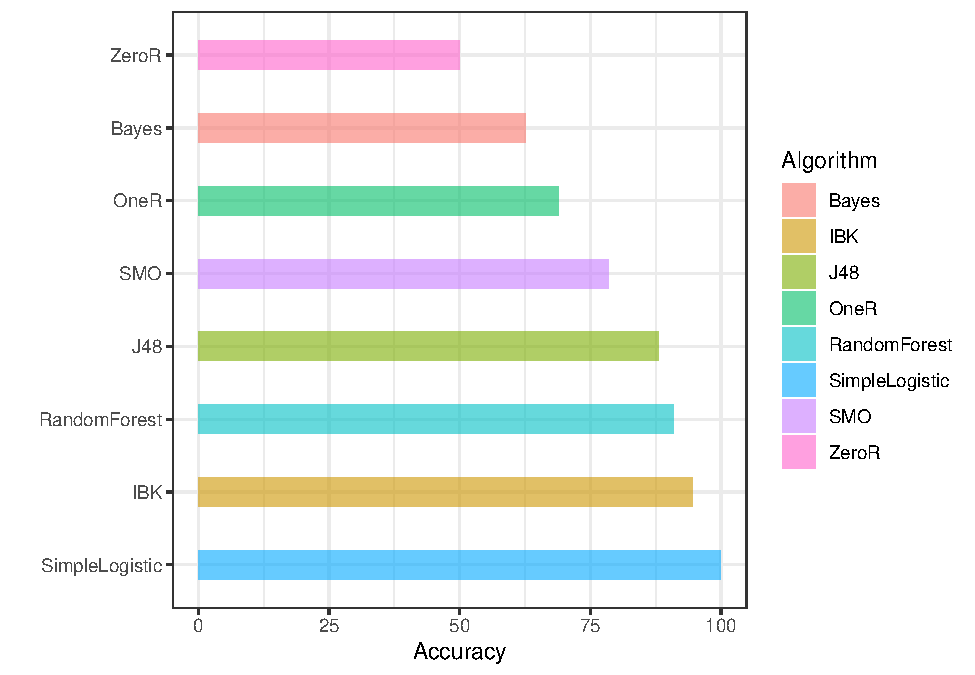
\includegraphics{Log_files/figure-latex/ml-1} 

}

\caption{The accuracy of the machine learning algorithms ordered from low to high.}\label{fig:ml}
\end{figure}

This plot shows a few interesting things, most notably the 100\%
accuracy of Simple logistic. The output in weka of the classification
using Simple logistic with 10 fold cross-validation shows a model for
each species. The model for the blue crabs shows 1.03 + {[}FL{]} * -0.6
+ {[}CW{]} * 0.31 + {[}BD{]} * -0.22. The model for the orange crabs
shows -1.03 + {[}FL{]} * 0.6 + {[}CW{]} * -0.31 + {[}BD{]} * 0.22. The
values in the model of the orange crabs are the values of the model of
the blue crabs times -1. The metrics used in the models are Front lobe
size, Carapace width and Body depth. The barplot also shows an exact
50\% accuracy for the ZeroR algorithm. This is expected since the data
has the same amount of blue crabs as orange crabs.

\newpage

\begin{Shaded}
\begin{Highlighting}[]
\NormalTok{metaalgorithms }\OtherTok{\textless{}{-}} \FunctionTok{read.csv}\NormalTok{(}\StringTok{"datafiles/meta ml.csv"}\NormalTok{)}
\NormalTok{metaalgorithms }\OtherTok{\textless{}{-}} \FunctionTok{data.frame}\NormalTok{(metaalgorithms)}

\FunctionTok{ggplot}\NormalTok{(metaalgorithms, }\FunctionTok{aes}\NormalTok{(}\AttributeTok{x =} \FunctionTok{reorder}\NormalTok{(Algorithm, }\FunctionTok{desc}\NormalTok{(Accuracy)), }\AttributeTok{y =}\NormalTok{ Accuracy, }\AttributeTok{fill =}\NormalTok{ Algorithm)) }\SpecialCharTok{+}
  \FunctionTok{geom\_bar}\NormalTok{(}\AttributeTok{stat=}\StringTok{"identity"}\NormalTok{, }\AttributeTok{alpha=}\NormalTok{.}\DecValTok{6}\NormalTok{, }\AttributeTok{width=}\NormalTok{.}\DecValTok{4}\NormalTok{) }\SpecialCharTok{+}
  \FunctionTok{coord\_flip}\NormalTok{() }\SpecialCharTok{+}
  \FunctionTok{xlab}\NormalTok{(}\StringTok{""}\NormalTok{) }\SpecialCharTok{+}
  \FunctionTok{theme\_bw}\NormalTok{()}
\end{Highlighting}
\end{Shaded}

\begin{center}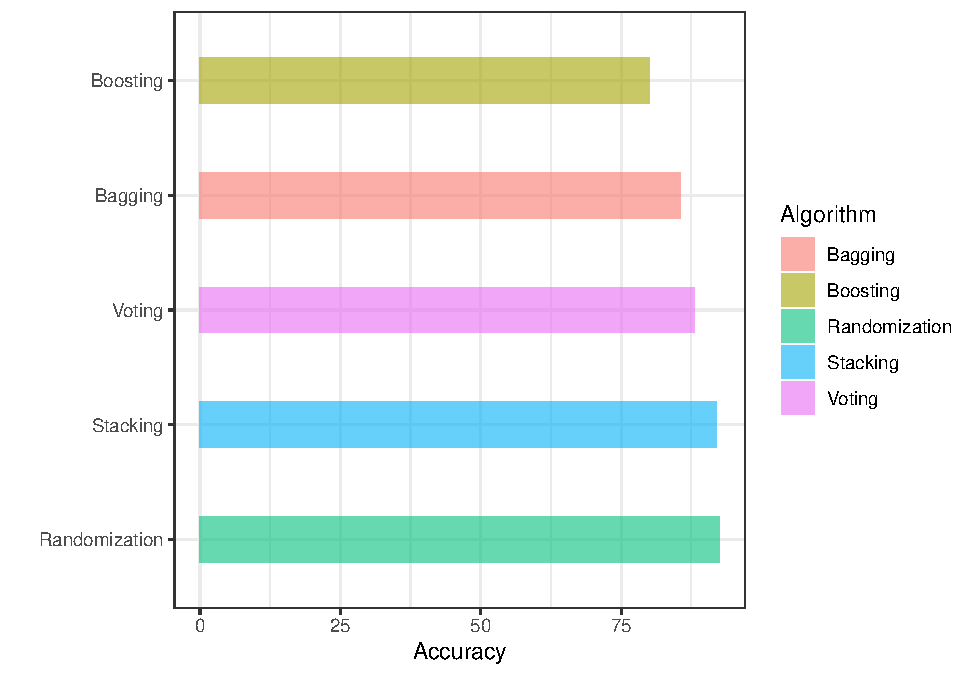
\includegraphics{Log_files/figure-latex/metalearners-1} \end{center}

\newpage

\hypertarget{discussion-and-future-research}{%
\subsection{Discussion and future
research}\label{discussion-and-future-research}}

The goal was to get the dataset ready for machine learning. The data was
analyzed and cleaned to make so it is ready to be used in machine
learning algorithms. The data does not contain many outliers. The data
points seem easy to classify since most plots show clear groups of blue
and orange crabs. As shown in figure 4, the gender of the crab could
also be a good attribute to help predict the species of crab. The data
also had to be cleaned. This was done by removing the index column,
since this column can not be used to help determine the species of crab.
It might also be a problematic attribute for some machine learning
algorithms. Then, the species column was moved to the last column, so
the machine learning algorithms will use this column as the class index.

Future research can be used to show more correlation between other
measurements. It can be researched whether or not the gender of the crab
could be predicted using these morphological measurements. Machine
learning use could also be improved by expanding the dataset, or getting
different amounts of blue or orange crabs, with different amounts of
male and female crabs.

\newpage

\end{document}
